% !TeX program = xelatex
\documentclass[a4paper,10pt]{article}

% ============================================================================
% ១. កញ្ចប់បណ្ណាល័យ និងការកំណត់ទំព័រ (Packages & Page Setup — តាមគំរូ ls_plan.tex)
% ============================================================================
\usepackage[a4paper, left=0.95cm, right=0.95cm, top=0.85cm, bottom=0.92cm, footskip=0.52cm]{geometry}
\usepackage{amsmath}
\usepackage{unicode-math}
\usepackage{fontspec}
\usepackage{longtable, array, multirow, colortbl}
\usepackage[table]{xcolor}
\usepackage{enumitem}
\usepackage{pifont}
\usepackage{fancyhdr}
\usepackage{tikz}
\usetikzlibrary{calc, arrows.meta, decorations.pathreplacing, patterns, positioning, babel}

\makeatletter
\let\@expl@@@mark@update@singlecol@structures@@\relax
\makeatother

% --- ប្រព័ន្ធស្វែងរកទីតាំងពុម្ពអក្សរស្វ័យប្រវត្តិ (Windows Local + Cloud Repo fonts/) ---
\providecommand{\NGSFindFonts}{%
  \IfFileExists{C:/Windows/Fonts/cambria.ttc}{%
    \def\NGSSysPath{C:/Windows/Fonts/}%
    \def\NGSUserPath{C:/Users/KIT/AppData/Local/Microsoft/Windows/Fonts/}%
  }{%
    \IfFileExists{./fonts/KhmerOSsiemreap.ttf}{\def\NGSSysPath{./fonts/}\def\NGSUserPath{./fonts/}}{%
    \IfFileExists{../fonts/KhmerOSsiemreap.ttf}{\def\NGSSysPath{../fonts/}\def\NGSUserPath{../fonts/}}{%
    \IfFileExists{../../fonts/KhmerOSsiemreap.ttf}{\def\NGSSysPath{../../fonts/}\def\NGSUserPath{../../fonts/}}{%
    \IfFileExists{../../../fonts/KhmerOSsiemreap.ttf}{\def\NGSSysPath{../../../fonts/}\def\NGSUserPath{../../../fonts/}}{%
    \IfFileExists{../../../../fonts/KhmerOSsiemreap.ttf}{\def\NGSSysPath{../../../../fonts/}\def\NGSUserPath{../../../../fonts/}}{%
    \IfFileExists{../../../../../fonts/KhmerOSsiemreap.ttf}{\def\NGSSysPath{../../../../../fonts/}\def\NGSUserPath{../../../../../fonts/}}{%
    \IfFileExists{../../../../../../fonts/KhmerOSsiemreap.ttf}{\def\NGSSysPath{../../../../../../fonts/}\def\NGSUserPath{../../../../../../fonts/}}{%
      \def\NGSSysPath{../../../../../../../fonts/}\def\NGSUserPath{../../../../../../../fonts/}%
    }}}}}}}%
  }%
}
\NGSFindFonts

% ============================================================================
% ២. កំណត់ពុម្ពអក្សរ (Fonts — តាមគំរូ ls_plan.tex)
% ============================================================================
\setmathfont[Path={\NGSSysPath}, FontIndex=1, Scale=1.02]{cambria.ttc}
\defaultfontfeatures{Ligatures=TeX}

\setmainfont[
  Path={\NGSUserPath},
  Extension=.ttf,
  Script=Khmer,
  BoldFont={KhmerOSsiemreap},
  BoldFeatures={FakeBold=1.8},
  ItalicFont={KhmerOSsiemreap},
  ItalicFeatures={FakeSlant=0.25},
  BoldItalicFont={KhmerOSsiemreap},
  BoldItalicFeatures={FakeBold=1.8, FakeSlant=0.25}
]{KhmerOSsiemreap}

\newfontfamily\muol[Path={\NGSUserPath}, Extension=.ttf, Script=Khmer]{KhmerOSmuollight}
\newfontfamily\Tacteing[Path={\NGSUserPath}, Extension=.TTF]{TACTENG}
\newfontfamily\TimesEn[Path={\NGSSysPath}, Extension=.ttf, BoldFont={timesbd}, ItalicFont={timesi}, BoldItalicFont={timesbi}]{times}
\newfontfamily\CalibriFont[Path={\NGSSysPath}, Extension=.ttf]{calibri}
\newfontfamily\CourierCirc[Path={\NGSSysPath}, Extension=.ttf]{cour}

\XeTeXlinebreaklocale "km"
\XeTeXlinebreakskip = 0pt plus 1pt minus 0.1pt

% ============================================================================
% ៣. ពណ៌ និងការតុបតែង (Colors & Styles)
% ============================================================================
\definecolor{stepbg}{HTML}{D9D9D9}
\definecolor{headgray}{HTML}{E6E6E6}
\definecolor{emphred}{HTML}{C00000}

\pagestyle{fancy}
\fancyhf{}
\renewcommand{\headrulewidth}{0pt}
\fancyfoot[R]{\CalibriFont\fontsize{9pt}{11pt}\selectfont\thepage}

\setlength{\parindent}{0pt}
\setlength{\parskip}{0pt}
\setlength{\tabcolsep}{4.5pt}
\setlength{\LTpre}{2pt}
\setlength{\LTpost}{2pt}

\newcolumntype{L}[1]{>{\raggedright\arraybackslash}p{#1}}
\newcolumntype{C}[1]{>{\centering\arraybackslash}p{#1}}

% ============================================================================
% ៤. ពាក្យបញ្ជាជំនួយ (Helper Macros)
% ============================================================================
\newcommand{\en}[1]{{\TimesEn #1}}
\newcommand{\enbf}[1]{{\TimesEn\bfseries #1}}
\newcommand{\khmflourish}{{\Tacteing\fontsize{15pt}{15pt}\selectfont 3}}
\newcommand{\wcirc}{{\CourierCirc\fontsize{9.5pt}{11pt}\selectfont o}}
\newcommand{\ditem}{{\fontsize{7.5pt}{10pt}\selectfont\ding{117}}\ }
\newcommand{\fiveE}[1]{\textcolor{emphred}{\CalibriFont\bfseries #1}}
\newcommand{\redsub}[1]{\textcolor{emphred}{#1}}
\newcommand{\timenote}[1]{\textcolor{emphred}{\textit{#1}}}
\newcommand{\stepheader}[1]{\multicolumn{3}{|c|}{\cellcolor{stepbg}\muol #1} \\ \hline}
\newcommand{\cfig}[1]{{\centering\vspace{3pt}#1\vspace{3pt}\par}}
\newcommand{\cnum}[1]{\mbox{\fontsize{10.5pt}{12pt}\selectfont\ding{\numexpr181+#1\relax}}}
\newcommand{\unit}[1]{\,\text{\en{#1}}}
\newcommand{\graybox}[1]{\colorbox{headgray}{\strut #1}}

% ============================================================================
% ៥. រូបភាព TikZ ស-ខ្មៅ សម្រាប់បង្រៀនលើក្ដារខៀន និងសន្លឹកកិច្ចការ (B&W Diagrams)
% ============================================================================

% ១. E1 Engage: អន្ទាក់ចំនួនគត់សេស និងលេខ 1, 2, 9
\newcommand{\figEngageDIVTwoThree}{%
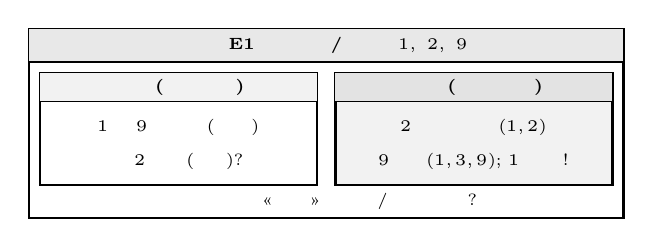
\begin{tikzpicture}[x=1cm, y=1cm, every node/.style={font=\fontsize{5.9pt}{7.8pt}\selectfont, text=black}]
  \draw[black, line width=0.9pt] (0,0) rectangle (7.55,2.40);
  \fill[gray!18] (0,1.98) rectangle (7.55,2.40);
  \draw[black, line width=0.6pt] (0,1.98) -- (7.55,1.98);
  \node at (3.775,2.19) {\textbf{បេសកកម្ម \en{E1}៖ អន្ទាក់ចំនួនគូ/សេស និងលេខ $1,\ 2,\ 9$}};

  % Student A
  \draw[black, line width=0.8pt] (0.14,0.42) rectangle (3.66,1.84);
  \fill[gray!10] (0.14,1.48) rectangle (3.66,1.84);
  \draw[black, line width=0.5pt] (0.14,1.48) -- (3.66,1.48);
  \node at (1.90,1.66) {\textbf{សិស្ស ក (មើលតាមគូ និងសេស)}};
  \node at (1.90,1.15) {$1$ និង $9$ ជាចំនួនបឋម (ព្រោះសេស)};
  \node at (1.90,0.72) {រីឯ $2$ មិនបឋម (ព្រោះគូ)?};

  % Student B
  \draw[black, line width=0.95pt, fill=gray!10] (3.89,0.42) rectangle (7.41,1.84);
  \fill[gray!22] (3.89,1.48) rectangle (7.41,1.84);
  \draw[black, line width=0.55pt] (3.89,1.48) -- (7.41,1.48);
  \node at (5.65,1.66) {\textbf{សិស្ស ខ (រាប់ចំនួនតួចែកពិត)}};
  \node at (5.65,1.15) {$2$ មានតួចែកតែពីរគត់ ($1, 2$)};
  \node at (5.65,0.72) {$9$ មានបី ($1,3,9$); $1$ មានតែមួយ!};

  \node at (3.775,0.21) {\textbf{សំណួរ៖} តើការកំណត់ «ចំនួនបឋម» អាស្រ័យលើគូ/សេស ឬលើចំនួនតួចែក?};
\end{tikzpicture}}

% ២. E2 Explore: ការបែងចែកតាមចំនួនតួចែក (1 តួចែក vs 2 តួចែក vs >2 តួចែក)
\newcommand{\figDivisorCountDIVTwoThree}{%
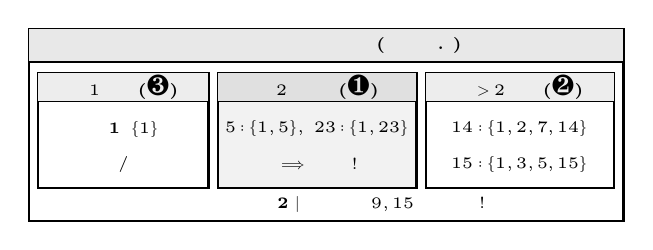
\begin{tikzpicture}[x=1cm, y=1cm, every node/.style={font=\fontsize{5.8pt}{7.6pt}\selectfont, text=black}]
  \draw[black, line width=0.9pt] (0,0) rectangle (7.55,2.44);
  \fill[gray!18] (0,2.02) rectangle (7.55,2.44);
  \draw[black, line width=0.6pt] (0,2.02) -- (7.55,2.02);
  \node at (3.775,2.23) {\textbf{ការបែងចែកចំនួនគត់ធម្មជាតិ តាមចំនួនតួចែក (សៀវភៅគោល ទំ.១៩)}};

  % Box 1: Unit 1
  \draw[black, line width=0.8pt] (0.12,0.42) rectangle (2.28,1.88);
  \fill[gray!14] (0.12,1.52) rectangle (2.28,1.88);
  \draw[black, line width=0.5pt] (0.12,1.52) -- (2.28,1.52);
  \node at (1.20,1.70) {\textbf{មាន $1$ តួចែក (\cnum{3})}};
  \node at (1.20,1.16) {លេខ $\mathbf{1}$៖ $\{1\}$};
  \node at (1.20,0.72) {មិនបឋម/មិនមែន};

  % Box 2: Primes
  \draw[black, line width=0.95pt, fill=gray!10] (2.40,0.42) rectangle (4.92,1.88);
  \fill[gray!24] (2.40,1.52) rectangle (4.92,1.88);
  \draw[black, line width=0.55pt] (2.40,1.52) -- (4.92,1.52);
  \node at (3.66,1.70) {\textbf{មាន $2$ តួចែកគត់ (\cnum{1})}};
  \node at (3.66,1.18) {$5:\{1,5\},\ 23:\{1,23\}$};
  \node at (3.66,0.72) {$\implies$ \textbf{ចំនួនបឋម}!};

  % Box 3: Composites
  \draw[black, line width=0.8pt] (5.04,0.42) rectangle (7.43,1.88);
  \fill[gray!14] (5.04,1.52) rectangle (7.43,1.88);
  \draw[black, line width=0.5pt] (5.04,1.52) -- (7.43,1.52);
  \node at (6.235,1.70) {\textbf{មាន $>2$ តួចែក (\cnum{2})}};
  \node at (6.235,1.18) {$14:\{1,2,7,14\}$};
  \node at (6.235,0.72) {$15:\{1,3,5,15\}$};

  \node at (3.775,0.21) {ចំនួនបឋមគូមានតែមួយគត់គឺ $\mathbf{2}$ $\mid$ ចំនួនសេសដូចជា $9, 15$ ជា\textbf{ចំនួនមិនបឋម}!};
\end{tikzpicture}}

% ៣. E4 Elaborate: លំហាត់គំរូ ទំ.១៩ (បឋមចន្លោះ 1-20 និង មិនបឋមសេសចន្លោះ 1-30)
\newcommand{\figModelsDIVTwoThree}{%
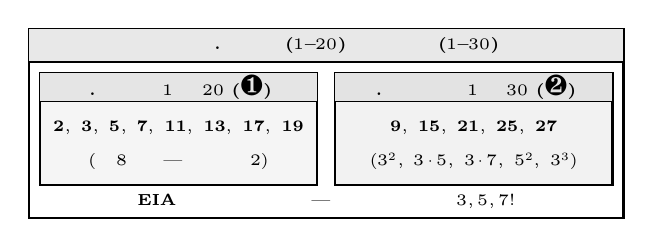
\begin{tikzpicture}[x=1cm, y=1cm, every node/.style={font=\fontsize{5.8pt}{7.6pt}\selectfont, text=black}]
  \draw[black, line width=0.9pt] (0,0) rectangle (7.55,2.40);
  \fill[gray!18] (0,1.98) rectangle (7.55,2.40);
  \draw[black, line width=0.6pt] (0,1.98) -- (7.55,1.98);
  \node at (3.775,2.19) {\textbf{លំហាត់គំរូ ទំ.១៩៖ ចំនួនបឋម ($1\text{--}20$) និងចំនួនមិនបឋមសេស ($1\text{--}30$)}};

  % Left: Primes between 1 and 20
  \draw[black, line width=0.85pt, fill=gray!8] (0.14,0.42) rectangle (3.66,1.84);
  \fill[gray!20] (0.14,1.48) rectangle (3.66,1.84);
  \draw[black, line width=0.5pt] (0.14,1.48) -- (3.66,1.48);
  \node at (1.90,1.66) {\textbf{ក. បឋមនៅចន្លោះ $1$ និង $20$ (\cnum{1})}};
  \node at (1.90,1.15) {$\mathbf{2,\ 3,\ 5,\ 7,\ 11,\ 13,\ 17,\ 19}$};
  \node at (1.90,0.72) {(មាន $8$ ចំនួន — រួមទាំងលេខគូ $2$)};

  % Right: Odd composites between 1 and 30
  \draw[black, line width=0.85pt, fill=gray!10] (3.89,0.42) rectangle (7.41,1.84);
  \fill[gray!22] (3.89,1.48) rectangle (7.41,1.84);
  \draw[black, line width=0.5pt] (3.89,1.48) -- (7.41,1.48);
  \node at (5.65,1.66) {\textbf{ខ. មិនបឋមសេសចន្លោះ $1$ និង $30$ (\cnum{2})}};
  \node at (5.65,1.15) {$\mathbf{9,\ 15,\ 21,\ 25,\ 27}$};
  \node at (5.65,0.72) {($3^2,\ 3\cdot 5,\ 3\cdot 7,\ 5^2,\ 3^3$)};

  \node at (3.775,0.21) {\textbf{\en{EIA}៖} ចំនួនសេសមិនមែនសុទ្ធតែបឋមទេ — ត្រូវពិនិត្យភាពចែកដាច់នឹង $3, 5, 7$!};
\end{tikzpicture}}

% ៣ខ. E5 Practice: តារាងលទ្ធផលកញ្ច្រែងអេរ៉ាតូស្ដែន < 50 (ប្រតិបត្តិ ទំ.១៩)
\newcommand{\figSieveFiftyDIVTwoThree}{%
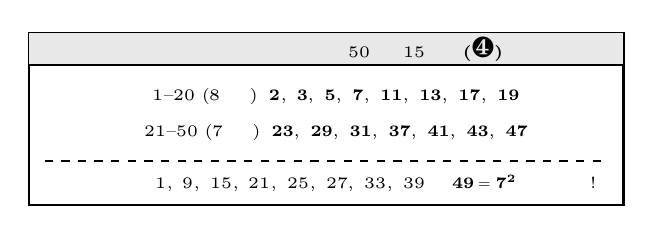
\begin{tikzpicture}[x=1cm, y=1cm, every node/.style={font=\fontsize{5.8pt}{7.5pt}\selectfont, text=black}]
  \draw[black, line width=0.9pt] (0,0) rectangle (7.55,2.18);
  \fill[gray!18] (0,1.78) rectangle (7.55,2.18);
  \draw[black, line width=0.6pt] (0,1.78) -- (7.55,1.78);
  \node at (3.775,1.98) {\textbf{លទ្ធផលកញ្ច្រែងអេរ៉ាតូស្ដែន៖ ចំនួនបឋមតូចជាង $50$ ទាំង $15$ ចំនួន (\cnum{4})}};
  \node at (3.775,1.38) {ជួរ $1\text{--}20$ ($8$ ចំនួន)៖ $\mathbf{2,\ 3,\ 5,\ 7,\ 11,\ 13,\ 17,\ 19}$};
  \node at (3.775,0.92) {ជួរ $21\text{--}50$ ($7$ ចំនួន)៖ $\mathbf{23,\ 29,\ 31,\ 37,\ 41,\ 43,\ 47}$};
  \draw[black, dashed, line width=0.45pt] (0.20,0.56) -- (7.35,0.56);
  \node at (3.775,0.28) {\textbf{ប្រយ័ត្នអន្ទាក់៖} លេខ $1,\ 9,\ 15,\ 21,\ 25,\ 27,\ 33,\ 39$ និង $\mathbf{49 = 7^2}$ សុទ្ធតែត្រូវឆូត!};
\end{tikzpicture}}

% ៤. E5 Evaluate: សំណួរវិនិច្ឆ័យ A-D
\newcommand{\figExitDIVTwoThree}{%
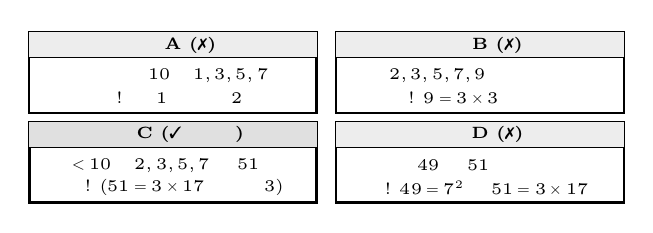
\begin{tikzpicture}[x=1cm, y=1cm, every node/.style={font=\fontsize{5.9pt}{7.6pt}\selectfont, text=black}]
  % Choice A
  \draw[black, line width=0.8pt] (0,1.14) rectangle (3.65,2.16);
  \fill[gray!14] (0,1.84) rectangle (3.65,2.16);
  \draw[black, line width=0.5pt] (0,1.84) -- (3.65,1.84);
  \node at (1.825,2.00) {\textbf{ជម្រើស \en{A} (\ding{55})}};
  \node at (1.825,1.61) {ចំនួនបឋមតូចជាង $10$ គឺ $1, 3, 5, 7$};
  \node at (1.825,1.33) {ខុស! ដាក់ $1$ និងភ្លេចលេខ $2$};

  % Choice B
  \draw[black, line width=0.8pt] (3.90,1.14) rectangle (7.55,2.16);
  \fill[gray!14] (3.90,1.84) rectangle (7.55,2.16);
  \draw[black, line width=0.5pt] (3.90,1.84) -- (7.55,1.84);
  \node at (5.725,2.00) {\textbf{ជម្រើស \en{B} (\ding{55})}};
  \node at (5.725,1.61) {$2, 3, 5, 7, 9$ សុទ្ធតែជាចំនួនបឋម};
  \node at (5.725,1.33) {ខុស! $9 = 3\times 3$ ជាចំនួនមិនបឋម};

  % Choice C (Correct)
  \draw[black, line width=1.05pt] (0,0) rectangle (3.65,1.02);
  \fill[gray!24] (0,0.70) rectangle (3.65,1.02);
  \draw[black, line width=0.6pt] (0,0.70) -- (3.65,0.70);
  \node at (1.825,0.86) {\textbf{ជម្រើស \en{C} (\ding{51} ត្រឹមត្រូវ)}};
  \node at (1.825,0.47) {បឋម $< 10$ គឺ $2, 3, 5, 7$ រីឯ $51$ មិនបឋម};
  \node at (1.825,0.19) {ត្រូវ! ($51 = 3\times 17$ ចែកដាច់នឹង $3$)};

  % Choice D
  \draw[black, line width=0.8pt] (3.90,0) rectangle (7.55,1.02);
  \fill[gray!14] (3.90,0.70) rectangle (7.55,1.02);
  \draw[black, line width=0.5pt] (3.90,0.70) -- (7.55,0.70);
  \node at (5.725,0.86) {\textbf{ជម្រើស \en{D} (\ding{55})}};
  \node at (5.725,0.47) {$49$ និង $51$ ជាចំនួនបឋម};
  \node at (5.725,0.19) {ខុស! $49=7^2$ និង $51=3\times 17$};
\end{tikzpicture}}

\begin{document}
\fontsize{10pt}{15.2pt}\selectfont

% ============================================================================
% ក្បាលរដ្ឋបាល (Administrative Header — តាមគំរូ ls_plan.tex)
% ============================================================================
{\centering
  {\muol\fontsize{11pt}{16pt}\selectfont ព្រះរាជាណាចក្រកម្ពុជា\par}
  {\muol\fontsize{11pt}{16pt}\selectfont ជាតិ សាសនា ព្រះមហាក្សត្រ\par}
  \vspace{-3pt}{\khmflourish\par}
}

\vspace{1pt}
{\muol\fontsize{10pt}{15.5pt}\selectfont
មន្ទីរអប់រំ យុវជន និងកីឡា ខេត្តកំពង់ធំ\par
ការិយាល័យអប់រំ យុវជន និងកីឡា ស្រុកកំពង់ស្វាយ\par
អនុវិទ្យាល័យព្រះក្រសាំង\par}

\vspace{2pt}
{\centering{\muol\fontsize{11.5pt}{17pt}\selectfont កិច្ចតែងការបង្រៀន\par}}
\vspace{2pt}

% --- ព័ត៌មានទូទៅ ---
{\hspace*{2.8cm}\renewcommand{\arraystretch}{1.08}
\begin{tabular}{@{}l@{\hspace{0.35cm}}p{2.9cm}@{\hspace{0.15cm}}c@{\hspace{0.25cm}}l@{}}
  - & មុខវិជ្ជា & : & គណិតវិទ្យា ថ្នាក់ទី៧ (ពីជគណិត) \\
  - & ចំណងជើងមេរៀន & : & មេរៀនទី២៖ តួចែកនិងពហុគុណ \\
  - & ចំណងជើងរង & : & ៣. ចំនួនបឋម និងចំនួនមិនបឋម (សៀវភៅគោល ទំ.១៩) \\
  - & រយៈពេល & : & ១ ម៉ោងសិក្សា (៥០ នាទី) \\
  - & បង្រៀនដោយ & : & ហុក ប៊ុនថែន \\
  - & កាលបរិច្ឆេទ & : & ថ្ងៃសៅរ៍ ទី១៤ ខែវិច្ឆិកា ឆ្នាំ២០២៦ \\
\end{tabular}\par}

\vspace{2pt}

% --- I. វត្ថុបំណង ---
{\muol\fontsize{10pt}{15.5pt}\selectfont \enbf{I.} វត្ថុបំណង\par}
\vspace{1pt}
{\renewcommand{\arraystretch}{1.10}
\begin{tabular}{@{}p{0.55cm}@{}p{2.35cm}@{\hspace{0.15cm}}c@{\hspace{0.25cm}}p{14.95cm}@{}}
  \hfill\wcirc\hspace{0.2cm} & វិជ្ជាសម្បទា & : & សិស្សប្រាប់បានពីនិយមន័យចំនួនបឋម ចំនួនមិនបឋម និងលក្ខណៈពិសេសនៃលេខ $1$ និងលេខ $2$ បានត្រឹមត្រូវតាមសៀវភៅគោលទំ.១៩ ។ \\
  \hfill\wcirc\hspace{0.2cm} & បំណិនសម្បទា & : & សិស្សបែងចែកចំនួនបឋមនិងចំនួនមិនបឋមតាមចំនួនតួចែក និងរកគ្រប់ចំនួនបឋមតូចជាង $50$ តាមកញ្ច្រែងអេរ៉ាតូស្ដែនលើសន្លឹកកិច្ចការបានត្រឹមត្រូវ ។ \\
  \hfill\wcirc\hspace{0.2cm} & ចរិយាសម្បទា & : & សិស្សមានទម្លាប់ផ្ទៀងផ្ទាត់តួចែកដោយម៉ត់ចត់ មិនសន្និដ្ឋានប្រញាប់ថា «សេសសុទ្ធតែបឋម» ឬ «$1$ ជាចំនួនបឋម» ឡើយ ។ \\
\end{tabular}\par}

\vspace{2pt}

% --- II. សម្ភារៈឧបទេស ---
{\muol\fontsize{10pt}{15.5pt}\selectfont \enbf{II.} សម្ភារៈឧបទេស\par}
\vspace{1pt}
\hspace*{0.55cm}$\bullet$\ សៀវភៅសិក្សាគោលថ្នាក់ទី៧ (ទំ.១៩ និងទំ.២៤) ក្ដារខៀន ដីស/ហ្វឺត និង\textbf{សន្លឹកកិច្ចការសិស្សបំពេញចន្លោះ ស-ខ្មៅ} (កូដ \en{DIV23} ទំព័រ ១--២ សម្រាប់សិស្ស និងទំព័រ ៣ ប្លង់ក្ដារខៀន/ចម្លើយគ្រូ — គ្មានប្រើ \en{LCD})\par

\vspace{2pt}

% --- III. វិធីសាស្រ្តបង្រៀន ---
{\muol\fontsize{10pt}{15.5pt}\selectfont \enbf{III.} វិធីសាស្រ្តបង្រៀន\par}
\vspace{1pt}
{\renewcommand{\arraystretch}{1.08}
\begin{tabular}{@{}p{0.55cm}@{}p{2.35cm}@{\hspace{0.15cm}}c@{\hspace{0.25cm}}p{14.95cm}@{}}
  \hfill$\bullet$\hspace{0.2cm} & គោលវិធី & : & សិស្សមជ្ឈមណ្ឌល (សន្លឹកកិច្ចការបំពេញចន្លោះជាគោល + ការពិភាក្សាជាក្រុមតូច ៣ នាក់) \\
  \hfill$\bullet$\hspace{0.2cm} & យុទ្ធវិធីបង្រៀន & : & គំរូស្ថាបនានិយម \en{5Es} រួមបញ្ចូល \textbf{ការធ្វើចំណាត់ថ្នាក់តាមចំនួនតួចែក} និង \textbf{កញ្ច្រែងអេរ៉ាតូស្ដែន (\en{Sieve of Eratosthenes})} \\
\end{tabular}\par}

\vspace{2pt}

% --- IV. ដំណើរការបង្រៀន ---
{\muol\fontsize{10pt}{15.5pt}\selectfont \enbf{IV.} ដំណើរការបង្រៀន\par}

{\renewcommand{\arraystretch}{1.14}
\begin{longtable}{|L{5.50cm}|L{7.90cm}|L{4.80cm}|}
\hline
\multicolumn{1}{|c|}{\cellcolor{headgray}\muol សកម្មភាពគ្រូ} &
\multicolumn{1}{c|}{\cellcolor{headgray}\muol ខ្លឹមសារមេរៀន} &
\multicolumn{1}{c|}{\cellcolor{headgray}\muol សកម្មភាពសិស្ស} \\
\hline
\endfirsthead

\hline
\multicolumn{1}{|c|}{\cellcolor{headgray}\muol សកម្មភាពគ្រូ} &
\multicolumn{1}{c|}{\cellcolor{headgray}\muol ខ្លឹមសារមេរៀន} &
\multicolumn{1}{c|}{\cellcolor{headgray}\muol សកម្មភាពសិស្ស} \\
\hline
\endhead

% ==================== ជំហានទី១ (2min) ====================
\stepheader{ជំហានទី១ \enbf{(}រដ្ឋបាលថ្នាក់\enbf{)}}
$\bullet$ ពិនិត្យវត្តមាន អនាម័យ និងសណ្ដាប់ធ្នាប់ថ្នាក់រៀន \par
$\bullet$ រៀបចំក្រុមតូច ៣ នាក់តាមតុ និងចែក\textbf{សន្លឹកកិច្ចការសិស្ស (\en{DIV23} ទំព័រ ១–២)}
&
$\bullet$ រដ្ឋបាលថ្នាក់ អនាម័យ និងវិន័យសិក្សា \par
$\bullet$ ចែកសន្លឹកកិច្ចការម្នាក់ ១ សន្លឹក សម្រាប់បំពេញតាមដំណាក់កាល \en{E1--E5}
&
$\circ$ ប្រធានថ្នាក់រាយការណ៍វត្តមានសិស្ស \par
$\circ$ ទទួលសន្លឹកកិច្ចការ សរសេរឈ្មោះ និងអង្គុយតាមក្រុម ៣ នាក់ \\
\hline

% ==================== ជំហានទី២ (9min: កំណែ <=3m + រំលឹក 3m + E1 3m) ====================
\stepheader{ជំហានទី២ \enbf{(}កិច្ចការផ្ទះ \enbf{+} ទំនាក់ទំនងមេរៀនថ្មី\enbf{)}}
\ditem \textbf{កំណែកិច្ចការផ្ទះ ($\le\text{\enbf{3\,min}}$)} \par
$\bullet$ ហៅសិស្សផ្ទៀងផ្ទាត់ចម្លើយលំហាត់ទំ.២៤ លេខ ១ និង លេខ ៣ លើក្ដារខៀនឆ្វេង
&
{\centering\redsub{កំណែកិច្ចការផ្ទះមេរៀនមុន (ទំ.២៤ លេខ ១ និង លេខ ៣)}\par}
$\bullet$ \textbf{លេខ ១៖} ក. $78+120\ (\div 2)$, ខ. $4\,140-720\ (\div 3)$, គ. $165+270\ (\div 5)$, ឃ. $5\,130-342\ (\div 9)$ \par
$\bullet$ \textbf{លេខ ៣៖} ពហុគុណនៃ $30$ គឺ $\mathbf{660}$ ($30\times 22$) និង $\mathbf{540}$ ($30\times 18$)
&
$\circ$ ផ្ទៀងចម្លើយលេខ ១ និងលេខ ៣ រួចកែចូលសៀវភៅ \\[3pt]

\ditem \textbf{រំលឹកមេរៀនទាក់ទង (\enbf{3min})} \par
$\bullet$ សួរ៖ «ចូររកតួចែកទាំងអស់នៃ $5,\ 14,\ 15$ និង $23$ — តើចំនួននីមួយៗមានតួចែកប៉ុន្មាន?»
&
{\centering\redsub{រំលឹកការរកតួចែកនៃចំនួនគត់}\par}
$\bullet$ តួចែកនៃ $5$៖ $\{1, 5\}$ ($2$ ចំនួន); នៃ $23$៖ $\{1, 23\}$ ($2$ ចំនួន) \par
$\bullet$ តួចែកនៃ $14$៖ $\{1, 2, 7, 14\}$ ($4$ ចំនួន); នៃ $15$៖ $\{1, 3, 5, 15\}$ ($4$ ចំនួន)
&
$\circ$ ឆ្លើយរាយតួចែក និងរាប់ឃើញ $5, 23$ មានតែ $2$ តួចែកគត់ \\[3pt]

\fiveE{E1 - Engage (3min)} \timenote{(កុំទាន់ផ្ដល់ចម្លើយ)} \par
\ditem \textbf{បេសកកម្មអន្ទាក់គូ/សេស និងលេខ $1, 2, 9$ (\en{E1})}
&
\redsub{បេសកកម្ម \en{E1}៖ តើលេខ $1,\ 2,\ 9$ មួយណាជាចំនួនបឋមពិតប្រាកដ?}
&
$\circ$ អានស្ថានភាពបញ្ហា \en{E1} \\[3pt]

$\bullet$ ឱ្យសិស្សពិភាក្សាជាគូរវាងអំណះអំណាងសិស្ស ក និងសិស្ស ខ លើ \en{E1}
&
$\bullet$ \textbf{សិស្ស ក៖} «$1$ និង $9$ ជាចំនួនបឋមព្រោះជាចំនួនសេស រីឯ $2$ មិនបឋមព្រោះជាចំនួនគូ» \par
$\bullet$ \textbf{សិស្ស ខ៖} «ត្រូវរាប់ចំនួនតួចែក! $2$ មានតួចែកតែពីរគត់ ($1, 2$) រីឯ $9$ មានតួចែកបី ($1,3,9$)!»
&
$\circ$ ពិភាក្សាជាគូ និងគូស \ding{51} ក្នុងប្រអប់ \en{E1} \\[3pt]

&
\cfig{\figEngageDIVTwoThree}
& \\
\hline

% ==================== ជំហានទី៣ (17min: E2 11m + E3 6m) ====================
\stepheader{ជំហានទី៣ \enbf{(}ខ្លឹមសារមេរៀនថ្មី\enbf{)}}
\fiveE{E2 - Explore (11min)} \par
$\bullet$ សរសេរចំណងជើងរង \textbf{៣. ចំនួនបឋម} លើក្ដារខៀន \par
\ditem \textbf{សកម្មភាព ១៖ ធ្វើចំណាត់ថ្នាក់តាមចំនួនតួចែក (ទំ.១៩, \enbf{5min}, \en{E2-A})}
&
៣. ចំនួនបឋម (សៀវភៅគោល ទំ.១៩) \par
$\bullet$ \textbf{ឧទាហរណ៍៖} $5$ និង $23$ មានតួចែក\textbf{តែពីរគត់} គឺ $1$ និងខ្លួនឯង $\implies$ ហៅថា \textbf{ចំនួនបឋម} \par
$\bullet$ $14$ និង $15$ មានតួចែក\textbf{ច្រើនជាងពីរ} $\implies$ ហៅថា \textbf{ចំនួនមិនបឋម}
&
$\circ$ រាប់ចំនួនតួចែកក្នុងតារាង \en{E2-A} ឃើញខុសគ្នារវាង $2$ តួចែក និង $>2$ តួចែក \\[3pt]

$\bullet$ ឱ្យសិស្សពិនិត្យតួចែកនៃលេខ $1$ និងលេខ $2$ ក្នុងតារាង \en{E2-A}
&
$\bullet$ លេខ $\mathbf{1}$ មានតួចែក\textbf{តែមួយគត់}គឺ $1$ $\implies$ មិនមែនបឋម ហើយក៏មិនមែនចំនួនមិនបឋមដែរ! \par
$\bullet$ លេខ $\mathbf{2}$ មានតួចែក $1$ និង $2$ ($2$ តួចែកគត់) $\implies$ $2$ ជា\textbf{ចំនួនបឋមគូតែមួយគត់}!
&
$\circ$ រកឃើញថា $1$ មានតួចែកតែមួយ រីឯ $2$ ជាបឋមគូតែមួយគត់ \\[3pt]

\ditem \textbf{សកម្មភាព ២៖ បំណកស្រាយកញ្ច្រែងអេរ៉ាតូស្ដែន $1\text{--}20$ (\enbf{6min}, \en{E2-B})} \par
$\bullet$ ឱ្យសិស្សអនុវត្តឆូតពហុគុណលើជួរលេខ $1\text{--}20$ ក្នុង \en{E2-B}
&
$\bullet$ \textbf{ជំហានកញ្ច្រែងអេរ៉ាតូស្ដែន ($1\text{--}20$)៖} (១) គូសខ្វែង $\times$ លេខ $1$; (២) គូសរង្វង់លេខ $2$ រួចឆូតពហុគុណនៃ $2$ ($4, 6, 8, \dots, 20$); (៣) គូសរង្វង់លេខ $3$ រួចឆូតពហុគុណនៃ $3$ ($9, 15$) $\implies$ ចំនួនសល់គឺ $\mathbf{2, 3, 5, 7, 11, 13, 17, 19}$!
&
$\circ$ អនុវត្តគូសខ្វែង $1$ និងឆូតពហុគុណនៃ $2, 3$ លើសន្លឹកកិច្ចការ \\[3pt]

&
\cfig{\figDivisorCountDIVTwoThree}
& \\[3pt]

% --- E3 Explain (6min) ---
\fiveE{E3 - Explain (6min)} \par
$\bullet$ ដឹកនាំសិស្សសង្ខេបនិយមន័យ «ជាទូទៅ» និង «សម្គាល់» (ទំ.១៩) លើ \en{E3}
&
$\bullet$ \textbf{ជាទូទៅ (ទំ.១៩)៖} \par
\hspace*{0.15cm}-- \textbf{ចំនួនបឋម} គឺជាចំនួនគត់ធំជាង $1$ ដែលមានតួចែក\graybox{តែពីរគត់} គឺ $1$ និងខ្លួនវា \par
\hspace*{0.15cm}-- \textbf{ចំនួនមិនបឋម} គឺជាចំនួនគត់ធំជាង $1$ ដែលមានតួចែក\graybox{ច្រើនជាងពីរ}
&
$\circ$ បំពេញប្រអប់និយមន័យចំនួនបឋម និងចំនួនមិនបឋមលើ \en{E3} \\[3pt]

$\bullet$ បញ្ជាក់ចំណុច\textbf{សម្គាល់ (ទំ.១៩)} អំពីលេខ «$1$» និងលេខ «$2$»
&
$\bullet$ \textbf{សម្គាល់ (ទំ.១៩)៖} «$\mathbf{1}$» មិនមែនជាចំនួនបឋម ហើយក៏មិនមែនជាចំនួនមិនបឋមដែរ ។ លេខ «$\mathbf{2}$» ជាចំនួនបឋមតូចបំផុត និងជាចំនួនបឋមគូតែមួយគត់ ។
&
$\circ$ កត់ចំណាំករណីពិសេសនៃលេខ $1$ និងលេខ $2$ \\[3pt]

$\bullet$ ភ្ជាប់\textbf{ធនាគារហេតុផល \cnum{1}--\cnum{2}} លើក្ដារខៀន និងសន្លឹកកិច្ចការ
&
\textbf{ធនាគារហេតុផល (\en{Warrant Bank})៖} \par
\cnum{1} \textbf{ចំនួនបឋម៖} ចំនួនគត់ $>1$ មានតួចែក $2$ គត់ ($1$ និងខ្លួនឯង) \par
\cnum{2} \textbf{ចំនួនមិនបឋម៖} ចំនួនគត់ $>1$ មានតួចែកច្រើនជាង $2$ (ចែកដាច់នឹងចំនួនផ្សេងទៀត)
&
$\circ$ ផ្ទៀងលេខកូដ \cnum{1}--\cnum{2} លើសន្លឹកកិច្ចការ \\[3pt]

$\bullet$ ភ្ជាប់\textbf{ធនាគារហេតុផល \cnum{3}--\cnum{4}} សម្រាប់លេខពិសេស និងកញ្ច្រែងអេរ៉ាតូស្ដែន
&
\cnum{3} \textbf{លេខពិសេស $1$ និង $2$៖} $1$ មានតួចែកតែ $1$ (មិនបឋម/មិនមែន); $2$ ជាបឋមគូតែមួយគត់ \par
\cnum{4} \textbf{កញ្ច្រែងអេរ៉ាតូស្ដែន ($<50$)៖} ឆូត $1$ និងពហុគុណនៃ $2, 3, 5, 7$ (ខុសពី $2, 3, 5, 7$)
&
$\circ$ ផ្ទៀងលេខកូដ \cnum{3}--\cnum{4} លើសន្លឹកកិច្ចការ \\
\hline

% ==================== ជំហានទី៤ (20min: E4 10m + E5 10m) ====================
\stepheader{ជំហានទី៤ \enbf{(}ពង្រីកចំណេះដឹង\enbf{)}}
\fiveE{E4 - Elaborate (10min)} \par
\ditem \textbf{លំហាត់គំរូ ក និង ខ តាមសៀវភៅគោល ទំ.១៩} \par
$\bullet$ ឱ្យសិស្សដោះស្រាយលំហាត់គំរូ ក (រកចំនួនបឋមនៅចន្លោះ $1$ និង $20$) លើ \en{E4}
&
{\muol លំហាត់គំរូ} \textbf{(សៀវភៅគោល ទំ.១៩)៖} \par
$\bullet$ \textbf{ក. ចំនួនបឋមនៅចន្លោះ $1$ និង $20$៖} គឺ \graybox{$2,\ 3,\ 5,\ 7,\ 11,\ 13,\ 17,\ 19$} ($8$ ចំនួន — សំអាង \cnum{1}, \cnum{3})
&
$\circ$ រាយចំនួនបឋមទាំង $8$ នៅចន្លោះ $1$ និង $20$ ដោយមិនភ្លេចលេខ $2$ \\[3pt]

$\bullet$ ឱ្យសិស្សដោះស្រាយលំហាត់គំរូ ខ (រកចំនួនមិនបឋមដែលជាចំនួនគត់សេសនៅចន្លោះ $1$ និង $30$)
&
$\bullet$ \textbf{ខ. ចំនួនមិនបឋមជាចំនួនគត់សេសនៅចន្លោះ $1$ និង $30$៖} គឺ \graybox{$9,\ 15,\ 21,\ 25,\ 27$} ព្រោះចែកដាច់នឹង $3$ ឬ $5$ ក្រៅពី $1$ និងខ្លួនឯង (\cnum{2})
&
$\circ$ ពិនិត្យចំនួនសេសពី $3$ ដល់ $29$ រកឃើញ $9, 15, 21, 25, 27$ មិនបឋម \\[3pt]

&
\cfig{\figModelsDIVTwoThree}
& \\[3pt]

$\bullet$ សួរសំណួរឆ្លុះបញ្ចាំង \textbf{\en{EIA Looking-Back} (1min)} លើការឈប់ឆូតត្រឹមពហុគុណនៃ $7$
&
\textbf{\en{EIA Looking-Back}៖} «ពេលរែងរកចំនួនបឋមតូចជាង $50$ ហេតុអ្វីយើងឆូតត្រឹមពហុគុណនៃ $2, 3, 5, 7$ មិនបាច់ឆូតពហុគុណនៃ $11$ ទៀត?» ($\to$ ព្រោះ $11\times 2, 11\times 3, 11\times 4$ ត្រូវឆូតរួចហើយ រីឯ $11\times 11 = 121 > 50$!)
&
$\circ$ ឆ្លុះបញ្ចាំងយល់មូលហេតុដែលកញ្ច្រែង $<50$ ឈប់ត្រឹមបឋម $7$ \\[3pt]

% --- E5 Evaluate (10min) ---
\fiveE{E5 - Evaluate (10min)} \par
\ditem \textbf{ប្រតិបត្តិជាក្រុមតូច ៣ នាក់ (4min, សន្លឹកកិច្ចការ \en{E5})} \par
$\bullet$ ឱ្យក្រុមសិស្សអនុវត្តកញ្ច្រែងអេរ៉ាតូស្ដែនលើតារាង $1\text{--}50$ ដើម្បីរកចំនួនបឋមតូចជាង $50$ (ប្រតិបត្តិ ទំ.១៩)
&
{\muol លំហាត់ប្រតិបត្តិ} \textbf{(សៀវភៅគោល ទំ.១៩ — រកចំនួនបឋមតូចជាង $50$)៖} \par
$\bullet$ អនុវត្តកញ្ច្រែង \cnum{4} បានចំនួនបឋមតូចជាង $50$ សរុប $\mathbf{15}$ ចំនួនគឺ៖ \par
$\mathbf{2,\ 3,\ 5,\ 7,\ 11,\ 13,\ 17,\ 19,}$ $\mathbf{23,\ 29,\ 31,\ 37,\ 41,\ 43,\ 47}$
&
$\circ$ សហការគ្នាឆូតតារាង $1\text{--}50$ រកឃើញបឋមទាំង $15$ ចំនួន \\[3pt]

&
\cfig{\figSieveFiftyDIVTwoThree}
& \\[3pt]

$\bullet$ ឱ្យក្រុមសិស្សផ្ទៀងផ្ទាត់និង\textbf{បិទបេសកកម្ម \en{E1} (2min)}
&
$\bullet$ \textbf{បិទបេសកកម្ម \en{E1}៖} \textbf{សិស្ស ខ} ត្រឹមត្រូវ! $2$ ជាចំនួនបឋមគូតែមួយគត់, $9$ ជាចំនួនមិនបឋមសេស, រីឯ $1$ មិនមែនបឋមនិងមិនមែនមិនបឋម (\cnum{1}--\cnum{3}) ។
&
$\circ$ បិទបេសកកម្ម \en{E1} ឃើញសិស្ស ខ ត្រឹមត្រូវ \\[3pt]

\ditem \textbf{សំណួរវិនិច្ឆ័យ \en{A--D} និងសំបុត្រចេញ (4min)} \par
$\bullet$ សរសេរជម្រើស \en{A--D} លើក្ដារខៀន
&
{\centering\textbf{សំណួរវិនិច្ឆ័យ \en{A--D}៖ តើប្រយោគមួយណាត្រឹមត្រូវ?}\par}
&
$\circ$ ពិនិត្យជម្រើសទាំង ៤ តាមកូដហេតុផល \cnum{1}--\cnum{4} \\[3pt]

$\bullet$ ឱ្យសិស្សគូសរង្វង់លើសន្លឹកកិច្ចការ និងលើកម្រាមដៃ ១--៤ ព្រមគ្នា
&
$\bullet$ វិភាគកំហុសក្នុងជម្រើស \en{A} (ដាក់ $1$/ភ្លេច $2$), \en{B} (ដាក់ $9$), \en{D} ($49=7^2,\ 51=3\times 17$)
&
$\circ$ គូសរង្វង់លើសន្លឹកកិច្ចការ និងលើកម្រាមដៃ ៣ (\textbf{ជម្រើស \en{C}}) \\[3pt]

$\bullet$ ឱ្យសិស្សបញ្ជាក់ហេតុផលដែលជម្រើស \en{C} ត្រឹមត្រូវតាមផលបូកខ្ទង់នៃ $51$
&
$\bullet$ \textbf{ផ្ទៀងផ្ទាត់ជម្រើស \en{C}៖} បឋម $<10$ គឺ $2, 3, 5, 7$ រីឯ $51$ មាន $5+1=6$ ចែកដាច់នឹង $3$ ($51=3\times 17$ ជាចំនួនមិនបឋម)
&
$\circ$ បញ្ជាក់ហេតុផលតាមភាពចែកដាច់នឹង $3$ និងកូដ \cnum{1}--\cnum{3} \\[3pt]

&
\cfig{\figExitDIVTwoThree}
& \\[3pt]

$\bullet$ បញ្ជាក់ចម្លើយត្រូវ (\textbf{ជម្រើស \en{C}}) និងឱ្យបំពេញ\textbf{សំបុត្រចេញ ៦០ វិនាទី}
&
$\bullet$ \textbf{សំបុត្រចេញ៖} ក្នុងចំណោម $1,\ 2,\ 21,\ 29,\ 49$ ចំនួនបឋមគឺ $\mathbf{2,\ 29}$ រីឯចំនួនមិនបឋមគឺ $\mathbf{21,\ 49}$ ($1$ ពិសេស) ។
&
$\circ$ បែងចែកចំនួនទាំង ៥ លើសំបុត្រចេញមុនបញ្ចប់ម៉ោង \\
\hline

% ==================== ជំហានទី៥ (<=2min) ====================
\stepheader{ជំហានទី៥ \enbf{(}កិច្ចការផ្ទះ \enbf{+} បណ្ដាំផ្ញើ\enbf{)}}
\timenote{ចំណាយពេលឱ្យតិចបំផុតកុំឱ្យលើស 2min} \par
$\bullet$ ណែនាំប្រអប់\textbf{កិច្ចការផ្ទះ}លើសន្លឹកកិច្ចការទំព័រ ២ (សៀវភៅគោល ទំ.២៤ លេខ ៤)
&
{\centering{\muol កិច្ចការផ្ទះ} \textbf{(សៀវភៅគោល ទំ.២៤ លេខ ៤)}\par} \par
$\bullet$ \textbf{លេខ ៤៖} គេមានចំនួន $11,\ 15,\ 17,\ 18,\ 19,\ 20,\ 21,\ 22,\ 23$ និង $29$ ៖ \par
\hspace*{0.25cm}ក. រកតួចែកនៃចំនួននីមួយៗ \qquad ខ. តើចំនួនណាខ្លះជាចំនួនបឋម?
&
$\circ$ គូសចំណាំលំហាត់ទំ.២៤ លេខ ៤ \\[3pt]

$\bullet$ ផ្ដាំផ្ញើឱ្យអានមុនចំណុច ៤. ការបំបែកមួយចំនួនជាផលគុណកត្តាបឋម (ទំ.២០)
&
$\bullet$ \textbf{បណ្ដាំផ្ញើ៖} អានមុន \textbf{៤. ការបំបែកមួយចំនួនជាផលគុណកត្តាបឋម} (សៀវភៅគោល ទំ.២០) លើឧទាហរណ៍ចំនួន $30$ ។
&
$\circ$ កត់ត្រាបណ្ដាំផ្ញើ ទុកសន្លឹកកិច្ចការក្នុងសៀវភៅ និងជម្រាបលាគ្រូ \\
\hline
\end{longtable}}

\vspace{6pt}
% --- ហត្ថលេខា (កាលបរិច្ឆេទត្រូវគ្នា ១០០% នឹងខាងលើ) ---
{\centering
\hspace*{5.2cm}\begin{minipage}{11.5cm}
  \centering
  ថ្ងៃសៅរ៍ ៥កើត ខែកត្តិក ឆ្នាំមមី អដ្ឋស័ក ពុទ្ធសករាជ ២៥៧០\par
  កំពង់ស្វាយ, ថ្ងៃទី១៤ ខែវិច្ឆិកា ឆ្នាំ២០២៦\par
  \vspace{2pt}
  {\muol គ្រូបង្រៀន\par}
  \vspace{32pt}
  \hfill{\muol ហុក ប៊ុនថែន}\hspace*{1.4cm}
\end{minipage}\par}

\end{document}
